\section{Architecture of the \dotNET Framework}
\label{sec:OverviewDotNetArchitecture}
\nomenclature{API}{Application Programming Interface}
The \dotNET Framework is Microsoft's platform for building, deploying, and running Web Services and applications. It is designed from scratch and has a consistent API providing support for component-based programs and Internet programming.
This new Application Programming Interface (API) has become an integral component of Windows. The \dotNET Framework was designed to fulfill the following objectives~\cite{Microsoft03-1}:

\begin{description}[noitemsep, style=nextline]
  \item[Consistency] Allow object code to be stored and executed locally, executed locally but Internet-distributed, or executed remotely and to make the developer experience consistent across a wide variety of types of applications, such as Windows-based applications and Web-based applications;
  \item[Operability] The ease of operation is enhanced by minimizing versioning conflicts and providing better software deployment support;
  \item[Security] All the code is executed safely, including code created by an unknown or semi-trusted third party;
  \item[Efficiency] The \dotNET Framework compiles applications to machine code before running thus eliminating the performance problems of scripted or interpreted environments;
  \item[Interoperability] Code based on the \dotNET Framework can integrate with other code because all communication is built on industry standards.
\end{description}

\begin{figure}
 \centering
 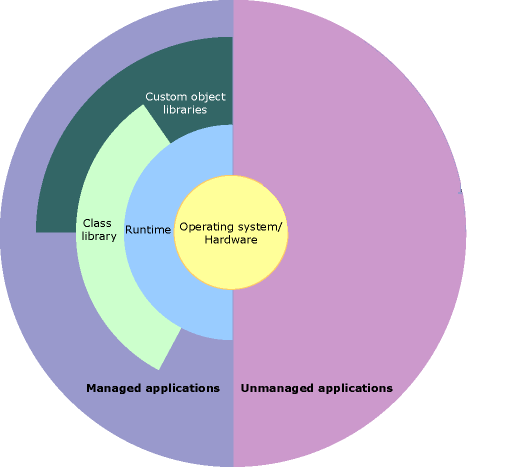
\includegraphics[style=thirdheight]{dotNET_context}
 \caption[Context of the \dotNET framework]{Context of the \dotNET Framework (Modified)~\cite{Microsoft03-1}}
 \label{fig:dotNET_context}
\end{figure}

\nomenclature{CLR}{Common Language Runtime}%
\nomenclature{CTS}{Common Type System}%
\nomenclature{CLS}{Common Language Specification}%
\nomenclature{FCL}{Framework Class Library}%
\nomenclature{CLI}{Common Language Infrastructure}%
The \dotNET Framework consists of two main components~\cite{Microsoft03-1}: the Common Language Runtime (CLR, simply called the \dotNET Runtime or Runtime for short) and the \dotNET Framework Class Library (FCL). 
The CLR is the foundation of the \dotNET Framework, executing the code and providing the core services such as memory management, thread management and exception handling. The CLR is described in more detail in \autoref{sec:clr}.
The class library, the other main component of the \dotNET Framework, is a comprehensive, object-oriented collection of reusable types that can be used to develop applications ranging from traditional command-line or graphical user interface (GUI) applications to applications such as Web Forms and XML Web services. \autoref{sec:fcl} describes the class libraries in more detail.

The code run by the runtime is in a format called Common Intermediate Language (CIL), further explained in~\autoref{sec:TheIntermediateLanguage}. The Common Language Infrastructure (CLI) is an open specification that describes the executable code and runtime environment that form the core of the Microsoft \dotNET Framework. \autoref{sec:cts} tells more about this specification.

\autoref{fig:dotNET_context} shows the relationship of the \dotNET Framework to other applications and to the complete system. The two parts, the class library and the runtime, are managed, \ie applications managed during execution. The operating system is in the core, managed and unmanaged applications operate on the hardware. The runtime can us other object libraries and the class library, but the other libraries can use the same class library them self.

Besides the Framework, Microsoft also provides a developer tool called the Visual Studio. This is an IDE with functionality across a wide range of areas allowing developers to build applications with decreased development time in comparison with developing applications using command line compilers.

\subsection{Version 2.0 of \dotNET}
\label{sec:Version2}
In November 2005, Microsoft released a successor of the \dotNET Framework. 
Major changes are the support for generics, the addition of nullable types, 64 bit support, improvements in the garbage collector, new security features and more network functionality.

Generics make it possible to declare and define classes, structures, interfaces, methods and delegates with unspecified or generic type parameters instead of specific types.
When the generic is used, the actual type is specified.
This allows for type-safety at compile-time.
Without generics, the use of casting or boxing and unboxing decreases performance.
By using a generic type, the risks and costs of these operations is reduced.

Nullable types allow a value type to have a normal value or a null value.
This null value can be useful for indicating that a variable has no defined value because the information is not currently available.

Besides changes in the Framework, there are also improvements in the four main Microsoft \dotNET programming languages (C\#, VB\dotNET, J\# and C++).
The language elements are now almost equal for all languages.
For instance, additions to the Visual Basic language are the support for unsigned values and new operators and additions to the C\# language include the ability to define anonymous methods thus eliminating the need to create a separate method.

A new Visual Studio 2005 edition was released to support the new Framework and functionalities to create various types of applications.
